\chapter{KẾT LUẬN VÀ HƯỚNG PHÁT TRIỂN}

\section{Kết luận chung về đề tài}
\label{sec:4.1_ket_luan_chung}

Đồ án đã hoàn thành trọn vẹn mục tiêu nghiên cứu, thiết kế và phát triển thành công hệ thống \textbf{Quản trị Tiến độ và Chi phí Dự án Logistics (GLPO)}. Bằng việc kết hợp sáng tạo giữa mô hình Trí tuệ nhân tạo Đồ thị dị thể và thuật toán Tối ưu hóa Lai đa mục tiêu, nghiên cứu đã giải quyết hiệu quả bài toán Lập lịch Dự án Hạn chế Tài nguyên (RCPSP) dưới tác động của rủi ro biến động ngẫu nhiên và ràng buộc tài chính phức tạp. Các đóng góp nổi bật của đề tài được tổng hợp trên cả hai khía cạnh lý luận khoa học và thực tiễn kỹ thuật.

\subsection{Đóng góp về mặt lý luận khoa học}
\label{sec:4.1.1_dong_gop_ly_luan}

Về mặt lý thuyết và phương pháp luận nghiên cứu, đồ án đóng góp ba luận điểm khoa học cốt lõi:

\begin{enumerate}
    \item \textbf{Mô hình hóa Đồ thị Dị thể:} Nghiên cứu đã tiên phong chuyển đổi toàn bộ bài toán quản lý dự án logistics từ các ma trận phẳng hai chiều truyền thống sang cấu trúc Đồ thị Dị thể $G = (V, E, \mathcal{T}_v, \mathcal{T}_e)$. Mô hình này biểu diễn tự nhiên mối quan hệ tương tác đa chiều giữa $3$ tập đỉnh ($V_{\text{Task}}$, $V_{\text{Resource}}$, $V_{\text{Shift}}$) và các tập cạnh phụ thuộc. Kết quả thực nghiệm khẳng định kiến trúc Heterogeneous Graph Transformer (HGT) bảo toàn tối đa thông tin ngữ cảnh, đạt độ chính xác dự báo vượt trội ($\text{MAE} = 0,98$ ngày, $\text{MAPE} = 3,21\%$, $R^2 = 0,942$) so với các kiến trúc học máy đồng thể (GCN, GAT) và mô hình bảng (XGBoost).
    
    \item \textbf{Giải pháp Học tự giám sát (SSL):} Nhằm vượt qua rào cản khan hiếm dữ liệu gán nhãn rủi ro trong quản lý chuỗi cung ứng, nghiên cứu đề xuất cơ chế Masked Autoencoder (MAE) trên đồ thị dị thể. Việc che khuất $25\%$ nút công việc và ép mô hình tái thiết lập đặc trưng giúp AI tự thụ cảm các quy luật lan truyền trễ mà không phụ thuộc vào nhãn thủ công, đảm bảo khả năng tổng quát hóa trên nhiều quy mô dự án.
    
    \item \textbf{Cơ chế Tối ưu hóa Lai:} Đề xuất mô hình phối hợp giữa Quy hoạch tuyến tính số nguyên hỗn hợp (MILP / CP-SAT) và Thuật toán Di truyền (GA). Việc sử dụng nghiệm nới lỏng từ MILP để tiêm $5\%$ "Hạt giống ưu tú" vào quần thể khởi tạo của GA giúp bộ giải duy trì tính khả thi $100\%$, tăng tốc độ hội tụ gấp $6,48$ lần (hội tụ tại thế hệ 45 so với thế hệ 412 của GA chuẩn) và giảm $84,57\%$ thời gian tính toán thực thi.
\end{enumerate}

\subsection{Đóng góp về mặt thực tiễn kỹ thuật}
\label{sec:4.1.2_dong_gop_thuc_tien}

Về mặt kỹ thuật hệ thống và triển khai thực địa, đề tài mang lại những giá trị ứng dụng cao cho các doanh nghiệp logistics:

\begin{enumerate}
    \item \textbf{Động cơ Truy vấn Đồ thị Đệ quy (Recursive CTE Engine):} Xây dựng giải pháp duyệt đồ thị phụ thuộc PDM trực tiếp trong nhân cơ sở dữ liệu quan hệ PostgreSQL thông qua biểu thức đệ quy (Recursive CTE). Giải pháp khắc phục triệt để bẫy hiệu năng $N+1$ Query của các framework ORM truyền thống, rút ngắn thời gian truy vấn tại quy mô $1.000$ nút từ $412,50$ ms xuống $14,20$ ms (tốc độ xử lý nhanh hơn $\mathbf{29,05\times}$), đáp ứng hoàn hảo yêu cầu phản hồi thời gian thực của ứng dụng Web.
    
    \item \textbf{Mô hình Phân ly 38 Loại Chi phí (G1--G7):} Đã hiện thực hóa mô hình tài chính đa tầng, phân rã ngân sách dự án thành 38 mục thuộc 7 nhóm chỉ số ($G_1$ đến $G_7$). Điều này hỗ trợ các nhà quản lý thực hiện chiến lược Ép tiến độ có mục tiêu, cân bằng tối ưu giữa chi phí làm thêm giờ, thuê nhà thầu phụ và tiền thưởng hoàn thành sớm ($3.000$ USD/tuần), minh chứng qua kết quả tối ưu ngân sách trên Case Study UniSA MFET 3008/5040 ($70.345$ USD).
    
    \item \textbf{Kiến trúc Microservices Triển khai Sản xuất:} Hệ thống được thiết kế theo kiến trúc vi dịch vụ (Microservices), đóng gói hoàn chỉnh bằng Docker và Docker Compose. Sự phân tách độc lập giữa phông nền Web UI (React + React-Flow), Backend API (FastAPI) và AI Service (PyTorch Geometric) giúp hệ thống đạt độ tin cậy cao, dễ dàng mở rộng và sẵn sàng tích hợp với các hệ thống ERP/WMS doanh nghiệp.
\end{enumerate}

\section{Đề xuất hướng phát triển}
\label{sec:4.2_huong_phat_trien}

Mặc dù đạt được những kết quả thực nghiệm ấn tượng, hệ thống vẫn còn một số điểm hạn chế cần tiếp tục hoàn thiện. Nhằm nâng cao hiệu năng và mở rộng phạm vi ứng dụng thực tế, nghiên cứu đề xuất ba hướng phát triển trọng tâm trong tương lai.

\subsection{Cải tiến Bộ Tối ưu hóa: Khắc phục điểm mù cục bộ bằng Thuật toán Di truyền Thích nghi (Adaptive GA)}
\label{sec:4.2.1_adaptive_ga}

Thực nghiệm tại Chương 3 chỉ ra rằng khi quy mô dự án bùng nổ ($|V| > 500$ nút) với mật độ ràng buộc tài nguyên nghiêm ngặt, thuật toán GA truyền thống vẫn chịu rủi ro suy giảm đa dạng di truyền, dẫn đến bẫy hội tụ sớm tại các cực trị cục bộ.

Để giải quyết triệt để bẫy tối ưu cục bộ, hướng nghiên cứu tiếp theo sẽ tập trung xây dựng \textbf{Thuật toán Di truyền Thích nghi (Adaptive Genetic Algorithm -- AGA)}. Trong AGA, xác suất lai ghép $P_c$ và xác suất đột biến $P_m$ không còn cố định mà được điều chỉnh động theo khoảng cách đa dạng nhiễm sắc thể trong từng thế hệ:
\begin{align}
P_c &= \begin{cases} 
k_1 \frac{f_{\max} - f'}{f_{\max} - f_{\text{avg}}}, & f' \geq f_{\text{avg}} \\
k_2, & f' < f_{\text{avg}}
\end{cases} \label{eq:adaptive_pc} \\
P_m &= \begin{cases} 
k_3 \frac{f_{\max} - f}{f_{\max} - f_{\text{avg}}}, & f \geq f_{\text{avg}} \\
k_4, & f < f_{\text{avg}}
\end{cases} \label{eq:adaptive_pm}
\end{align}
trong đó $f_{\max}$, $f_{\text{avg}}$ là giá trị thích nghi lớn nhất và trung bình của quần thể, $f'$ là giá trị thích nghi của cá thể trội hơn khi lai ghép, và $f$ là giá trị thích nghi của cá thể bị đột biến. Cơ chế thích nghi này giúp tự động kích hoạt xác suất đột biến cao khi quần thể rơi vào trạng thái bế tắc, đẩy quần thể thoát khỏi điểm mù cục bộ và tìm kiếm nghiệm tối ưu toàn cục.

\subsection{Nâng cấp Kiến trúc Học máy Đồ thị: Áp dụng cơ chế Chú ý Nâng cao như Graphormer}
\label{sec:4.2.2_graphormer}

Mô hình Heterogeneous Graph Transformer (HGT) hiện tại phụ thuộc chủ yếu vào các liên kết kề trực tiếp. Đối với các dự án logistics có chuỗi phụ thuộc kéo dài hàng trăm bước nhảy, việc luân chuyển thông tin qua nhiều lớp GNN dễ gặp phải hiện tượng nghẽn thông tin và san bằng đặc trưng.

Hướng phát triển tiếp theo sẽ tiến hành nâng cấp mô hình AI lên kiến trúc \textbf{Graphormer} \cite{ying2021graphormer} -- một biến thể Transformer nâng cao chuyên biệt cho đồ thị. Graphormer tích hợp ba cơ chế mã hóa cấu trúc vượt trội:
\begin{itemize}
    \item \textbf{Spatial Encoding (Mã hóa Không gian):} Đo đạc khoảng cách đường đi ngắn nhất $d(v_i, v_j)$ giữa hai nút bất kỳ trong đồ thị AON, cho phép các công việc ở thượng nguồn tương tác trực tiếp với hạ nguồn mà không bị suy giảm tín hiệu.
    \item \textbf{Centrality Encoding (Mã hóa Mức độ Trung tâm):} Nhúng chỉ số trung tâm bậc vào ma trận Attention, giúp mô hình tập trung tối đa vào các nút thắt giao thoa giữa nhiều luồng công việc.
    \item \textbf{Edge Encoding (Mã hóa Cạnh Dị thể):} Biểu diễn loại liên kết PDM (FS, SS, FF) và tài nguyên tiêu thụ trực tiếp vào tích vô hướng của cơ chế Self-Attention.
\end{itemize}

Sơ đồ concept tổng thể của kiến trúc Cơ chế Chú ý Nâng cao (Graphormer Advanced Attention) đề xuất được minh họa tại Hình \ref{fig:advanced_attention}.

\begin{figure}[H]
\centering
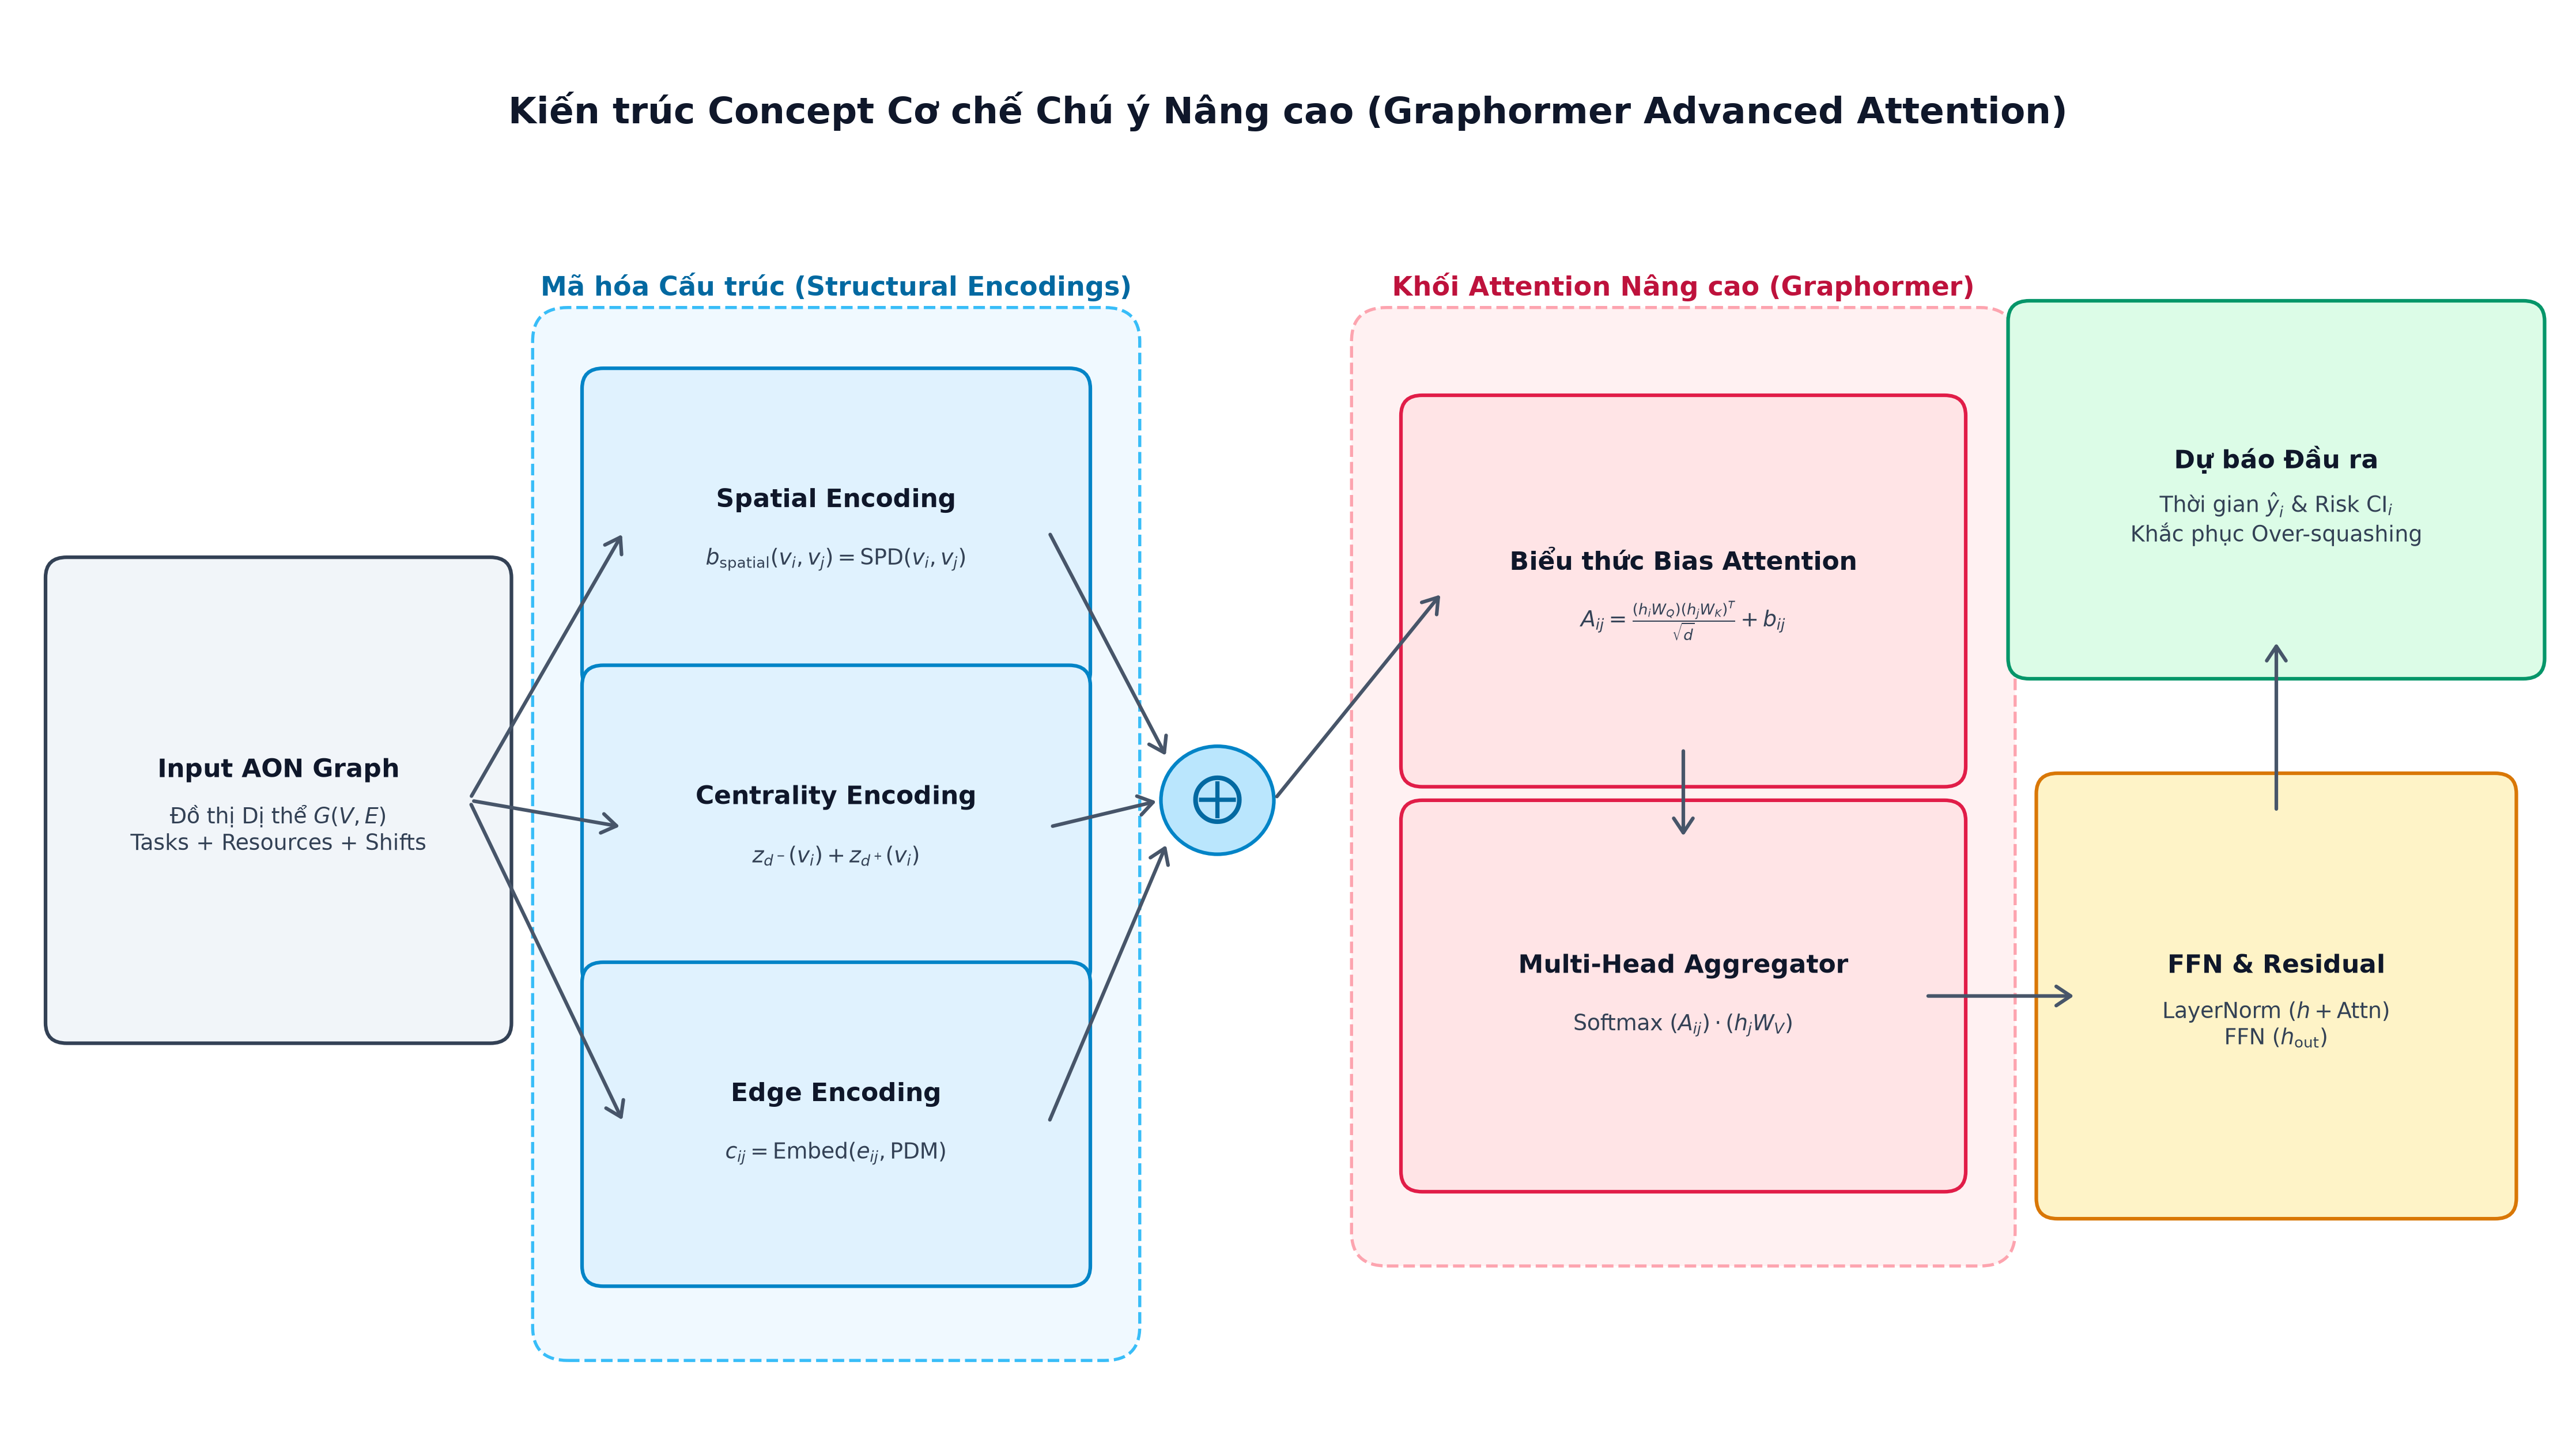
\includegraphics[width=0.95\linewidth]{image/hinh4_1_advanced_attention.png}
\caption{Sơ đồ Concept đề xuất kiến trúc Cơ chế Chú ý Nâng cao (Graphormer Advanced Attention) thay thế cho kiến trúc HGT cơ bản.}
\label{fig:advanced_attention}
\end{figure}

\subsection{Mở rộng Dữ liệu Huấn luyện: Thu thập dữ liệu thực tế tăng tính Tổng quát}
\label{sec:4.2.3_data_scaling}

Mặc dù hệ thống đã được thử nghiệm và đối chuẩn thành công trên các bộ dữ liệu quốc tế như UniSA MFET 3008/5040 và PSPLIB/DSLIB, các tập dữ liệu này vẫn mang tính chất mô phỏng kỹ thuật chuẩn mực.

Trong tương lai, nghiên cứu hướng tới việc mở rộng thu thập dữ liệu thi công thực tế từ các doanh nghiệp Logistics và Tập đoàn Xây dựng hạ tầng lớn. Việc thu thập chuỗi dữ liệu thời gian thực từ thiết bị giám sát hành trình GPS, hệ thống quản lý kho WMS và dữ liệu thời tiết lịch sử sẽ giúp:
\begin{enumerate}
    \item \textbf{Huấn luyện Mô hình Học sâu Chuỗi thời gian:} Kết hợp HGT/Graphormer với mạng LSTM/GRU để dự báo sự biến động chi phí nhiên liệu, cước vận tải và năng lực cung ứng nguyên vật liệu theo mùa.
    \item \textbf{Xây dựng Nền tảng SaaS và Đồng bộ ERP:} Đóng gói phân hệ AI thành các API chuẩn RESTful/GraphQL, hỗ trợ tích hợp Plug-and-Play vào các phần mềm quản trị phổ biến như Microsoft Project, Primavera P6 và SAP ERP.
\end{enumerate}
